\documentclass[utf8]{ctexbeamer}

\usepackage{graphicx}
\usepackage{listings}
\usepackage{tcolorbox}
\usepackage{tabularx}
\usepackage{hyperref}

\lstset{
    basicstyle=\ttfamily\scriptsize, 
    commentstyle=\color{black!37.3!green},
    keywordstyle=\color{blue},
    breaklines=true,
    numbers=left, 
    numberstyle=\tiny\color{gray}, 
    frame=single,
}

\title{平衡树}
\author{史浩诚}
\date{\today}

\begin{document}
	\frame{\titlepage}
	
    \begin{frame}
        \frametitle{目录}
        \tableofcontents 
    \end{frame}

    \section{二叉搜索树}

	\begin{frame}
		\frametitle{二叉搜索树}
        \begin{itemize}
            \item 二叉搜索树(Binary Search Tree),又名二叉排序树(Binary Sort Tree),简称BST
            \item 二叉搜索树是一个二叉树,每个结点都有一个权值(数据),且每个结点左子树所有结点的权值都小于此结点的权值,每个结点右子树所有结点的权值都大于此结点的权值。
            \item 二叉搜索树的中序遍历是有序的。
            \item 二叉搜索树支持很多操作。
        \end{itemize}
        例:
        \begin{figure}
            \centering
            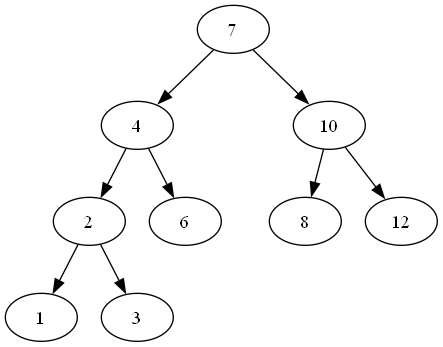
\includegraphics[width=0.5\textwidth]{images/BST.png}
        \end{figure}

	\end{frame}

    \begin{frame}
        \frametitle{\href{https://www.luogu.com.cn/problem/P3369}{P3369 【模板】普通平衡树}}
        \framesubtitle{\textcolor[RGB]{52, 152, 219}{提高+/省选−}}
        您需要动态地维护一个可重集合 $M$,并且提供以下操作:
        \begin{enumerate}
            \item 向 $M$ 中插入一个数 $x$。
            \item 从 $M$ 中删除一个数 $x$(若有多个相同的数,应只删除一个)。
            \item 查询 $M$ 中有多少个数比 $x$ 小,并且将得到的答案加一。
            \item 查询如果将 $M$ 从小到大排列后,排名位于第 $x$ 位的数。
            \item 查询 $M$ 中 $x$ 的前驱(前驱定义为小于 $x$,且最大的数)。
            \item 查询 $M$ 中 $x$ 的后继(后继定义为大于 $x$,且最小的数)。
        \end{enumerate}
        对于操作 3,5,6,\textbf{不保证}当前可重集中存在数 $x$。
    \end{frame}

    \begin{frame}[fragile]
        \frametitle{二叉搜索树}
        二叉搜索树支持以上操作。

        二叉搜索树的每个结点包含一下信息:
        \begin{lstlisting}[language=C++]
    Type val; // 值(数据)
    int cnt = 1; // cnt:val出现了cnt次
    size_t size = 1; // size:子树大小
    Node *leftSon = nullptr; // 左子树
    Node *rightSon = nullptr; // 右子树
        \end{lstlisting}
    \end{frame}
    
    \begin{frame}[fragile]
        \frametitle{插入}
        从根结点开始向下遍历,直到找到一个与插入值相同的结点或者是空结点。
        \begin{lstlisting}[language=C++]
void insert(Node *&cur, Type val) {
    if (!cur) {
        cur = new Node(val);
        return;
    }
    if (cur->val == val) {
        cur->cnt++;
    } else if (cmp(val, cur->val)) { 
            // val < cur->val
        insert(cur->leftSon, val);
    } else {
        insert(cur->rightSon, val);
    }
    cur->update();
}
        \end{lstlisting}
    \end{frame}

    \begin{frame}[fragile]
        \frametitle{查询排名}
        \begin{lstlisting}[language=c++]
size_t _queryRank(Node *&cur, Type val) {
    if (!cur) return 1; // 空树中任何值排名都为1
    size_t leftSonSize = cur->leftSon ? cur->leftSon->size : 0;
    if (val == cur->val) {
        return leftSonSize + 1;
    }
    if (cmp(val, cur->val)) { // val < cur->val
        return _queryRank(cur->leftSon, val);
    } else {
        return leftSonSize + cur->cnt + _queryRank(cur->rightSon, val);
    } // 在右子树中查询排名,加上当前结点的个数和左子树大小
}
        \end{lstlisting}
    \end{frame}

    \begin{frame}[fragile]
        \frametitle{查询第K小}
        \begin{lstlisting}[language=c++]
Type _queryKth(Node *&cur, size_t rank) {
    size_t leftSonSize = cur->leftSon ? cur->leftSon->size : 0;
    if (rank <= leftSonSize) {
        return _queryKth(cur->leftSon, priority);
    } else if (rank <= leftSonSize + cur->cnt) {
        return cur->val;
    } else if (rank <= cur->size) {
        return _queryKth(cur->rightSon, rank - leftSonSize - cur->cnt);
    }
}
        \end{lstlisting}       
    
    \end{frame}

    \begin{frame}[fragile]
        \frametitle{查询前驱}
        \begin{lstlisting}[language=c++]
Type _predecessor(Node *&cur, Type val) {
    if (cmp(val, cur->val) || val == cur->val) { 
        // 如果val与当前结点val相同或者小于当前结点val都需要在左子树继续查找前驱
        if (cur->leftSon) return _predecessor(cur->leftSon, val);
        else throw NoSuchValueException("No lesser value in the tree");
    } // 否则val大于当前结点val
    if (cur->rightSon) { 
        try { // 若有右子树,先在右子树中查找
            return _predecessor(cur->rightSon, val);
        } catch(const NoSuchValueException &e) {
            return cur->val;
        }
    }
    return cur->val; // 没有右子树返回当前结点
}
        \end{lstlisting}
    \end{frame}

    \begin{frame}[fragile]
        \frametitle{查询后继}
        \begin{lstlisting}[language=c++]
Type _successor(Node *&cur, Type val) {
    if (cmp(cur->val, val) || cur->val == val) {
        if (cur->rightSon) return _successor(cur->rightSon, val);
        else throw NoSuchValueException("No greater value in the tree");
    }
    if (cur->leftSon) {
        try {
            return _successor(cur->leftSon, val);
        } catch(const NoSuchValueException &e) {
            return cur->val;
        }
    }
    return cur->val;
}
        \end{lstlisting}
        查询x的前驱还有其他简单的方法,先查询x的排名,再查询排名-1的数是多少即为x的前驱,后继也是同理。
    \end{frame}

    \begin{frame}
        \frametitle{时间复杂度}
        \noindent
        \begin{minipage}[b]{0.5\textwidth}
            二叉搜索树的操作的时间复杂度都是取决于操作结点的深度,而二叉搜索树在最坏情况下退化成一条链的形状时,树的深度则会变成结点数$n$,所以二叉搜索树单次操作时间复杂度为$O(n)$
            
            最坏情况例子:先插入5,再插入4,再插入3,再插入2,再插入1,此时树为一条链

            那么降低时间复杂度,关键是在降低树的高度,使树“平衡”。
        \end{minipage}
        \hfill
        \begin{minipage}[b]{0.4\textwidth}
            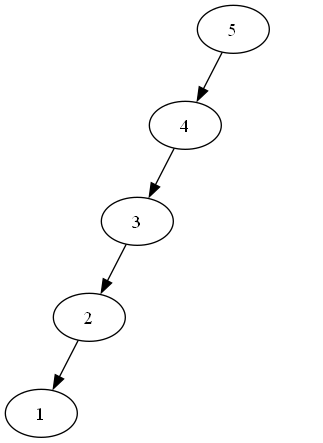
\includegraphics[width=\linewidth]{images/BST_list.png}
        \end{minipage}
        
    \end{frame}

    \section{Treap}

    \begin{frame}
        \frametitle{Treap}
        Treap,即Tree+heap组合而来,意思即为树堆,其中树指的就是二叉搜索树。
        \begin{tcolorbox}[colframe=blue,title=二叉堆]
            二叉堆是一棵二叉树,每个结点有一个值,每个结点的子结点的值都小于(或大于)当前结点的值
        \end{tcolorbox}
        Treap通过在二叉搜索树每个结点上加上一个随机生成$priority$,每个结点的子结点的$priority$都小于(或大于)当前结点的$priority$,来使得树平衡。
        \begin{figure}
            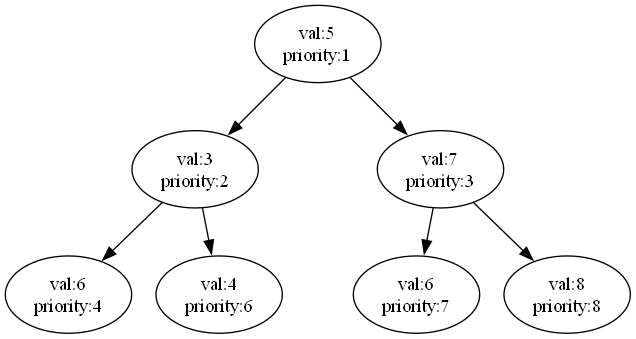
\includegraphics[width=0.5\textwidth]{images/Treap.png}
        \end{figure}
    \end{frame}

    \subsection{旋转Treap}

    \begin{frame}
        \frametitle{旋转}
        Treap插入结点有可能破坏堆的性质。

        Treap可以通过旋转操作来维护堆的性质,这种Treap称为旋转Treap。
        
        旋转操作,指不改变BST的性质的前提下,调整树的结构。
        旋转操作有两种:左旋和右旋。旋转操作并不是Treap独有的,其它一些平衡树也有旋转操作。

        Treap的旋转使得BST满足堆的性质。 
        
        首先介绍右旋
    
    \end{frame}

    \begin{frame}
        \frametitle{右旋}

        \begin{figure}
            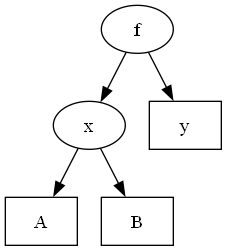
\includegraphics[width=0.3\textwidth]{images/right_rotate0.png}
            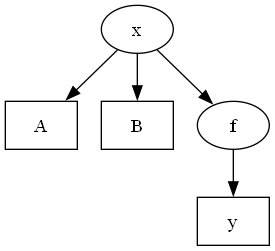
\includegraphics[width=0.3\textwidth]{images/right_rotate1.png}
            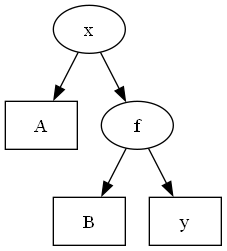
\includegraphics[width=0.3\textwidth]{images/right_rotate2.png}
        \end{figure}
        当左子树 $x$ 的 $priority$ 大于当前结点 $f$ 的 $priority$ 时,
        需要进行右旋,右旋后,$f$ 成为 $x$ 的右子树,满足了对的性质。

        由BST的性质可知,$A < x < B < f < y$,$A, B, y$ 代表的是$A, B, y$结点及其子树。
        
        我们先将$x$作为根结点,得到图2,但此时$x$有$3$个子结点,而$f$只有一个子结点,所以考虑将$B$子树移动成为$f$的左子树。    
    \end{frame}

    \begin{frame}[fragile]
        \frametitle{右旋}
    
        \begin{figure}
            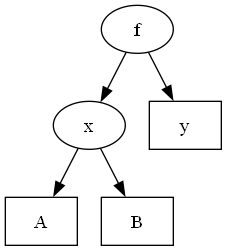
\includegraphics[width=0.3\textwidth]{images/right_rotate0.png}
            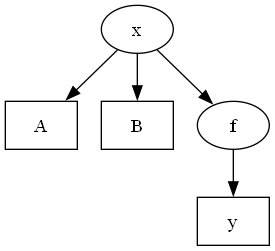
\includegraphics[width=0.3\textwidth]{images/right_rotate1.png}
            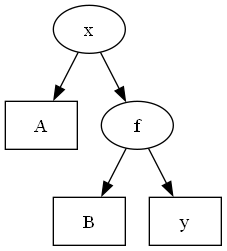
\includegraphics[width=0.3\textwidth]{images/right_rotate2.png}
        \end{figure}
    
        \begin{lstlisting}[language=c++]
void rightRotate(Node *&cur) {
    Node *tmp = cur->leftSon; // x
    cur->leftSon = tmp->rightSon; // 移动 B 子树
    tmp->rightSon = cur; // 移动 f
    cur->update(), tmp->update(); // 更新
    cur = tmp; // 将根改成 tmp(x结点)
}
        \end{lstlisting}
    \end{frame}

    \begin{frame}[fragile]
        \frametitle{左旋}
        \begin{figure}
            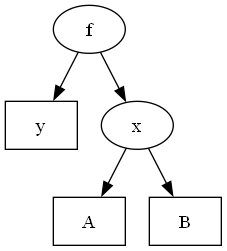
\includegraphics[width=0.3\textwidth]{images/left_rotate0.png}
            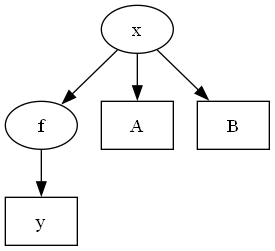
\includegraphics[width=0.3\textwidth]{images/left_rotate1.png}
            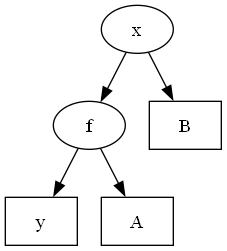
\includegraphics[width=0.3\textwidth]{images/left_rotate2.png}
        \end{figure}
    
        \begin{lstlisting}[language=c++]
void leftRotate(Node *&cur) {
    Node *tmp = cur->rightSon;
    cur->rightSon = tmp->leftSon;
    tmp->leftSon = cur;
    cur->update(), tmp->update();
    cur = tmp;
}
        \end{lstlisting}
    \end{frame}

    \begin{frame}[fragile]
        \frametitle{插入}满足堆的性质,
        具体来说,新建结点后,假如子结点大于当前结点的$priority$,则将其旋转,通过一层层的递归,将其旋转到合适的位置。相比于普通BST的插入,代码只多了两个if语句。
        \begin{lstlisting}[language=c++]
void insert(Node *&cur, Type val) {
    if (!cur) {
        cur = new Node(val);
        return;
    }
    if (cur->val == val) {
        cur->cnt++;
    } else if (cmp(val, cur->val)) { // val < cur->val
        insert(cur->leftSon, val);
        if (cur->leftSon->priority > cur->priority) {
            rightRotate(cur);
        }
    } else {
        insert(cur->rightSon, val);
        if (cur->rightSon->priority > cur->priority) {
            leftRotate(cur);
        }
    }
    cur->update();
}
        \end{lstlisting}
    \end{frame}

    \begin{frame}[fragile]
        \frametitle{删除}
        Treap在删除某个结点时:
        \begin{enumerate}
            \item 假如这个结点没有子结点,直接删除即可。
            \item 有一个子结点时,把当前结点改为子结点。
            \item 有两个子结点时,将$priority$较大的结点旋转上来,此时要删除的结点成为了当前结点的子结点,递归删除。
        \end{enumerate}
        \begin{lstlisting}[language=c++]
bool _erase(Node *&cur, Type val) {
    if (cur == nullptr) return false;
    if (val < cur->val) {
        if (_erase(cur->leftSon, val)) {
            cur->update();
            return true;
        }
        return false;
    } else if (val > cur->val) {
        if (_erase(cur->rightSon, val)) {
            cur->update();
            return true;
        }
        return false;
    }
        \end{lstlisting}
    \end{frame}

    \begin{frame}[fragile]
        \frametitle{删除}
        \begin{lstlisting}[language=c++]
    if (cur->cnt > 1) {
        cur->cnt--, cur->size--;
    } else if (cur->leftSon && cur->rightSon) {
        if (cur->leftSon->priority < cur->rightSon->priority) {
            rightRotate(cur);
            _erase(cur->rightSon, val);
        } else {
            leftRotate(cur);
            _erase(cur->leftSon, val);
        }
        cur->update();
    } else if (cur->leftSon) {
        Node* tmp = cur;
        cur = tmp->leftSon;
        delete tmp;
    } else if (cur->rightSon) {
        Node* tmp = cur;
        cur = tmp->rightSon;
        delete tmp;
    } else {
        delete cur;
        cur = nullptr;
    }
    return true;
}
        \end{lstlisting}
    \end{frame}

    \begin{frame}
        \frametitle{建树}
        由一个序列建树,我们可以直接将序列的每项一次次的插入,这样的时间复杂度为$O(n\log n)$
        但如果这个序列有序,则我们可以由以下两种方法建树:

        方法一:通过递归,每次选中间项为根,再递归建左子树和右子树,在建的时候保证$priority$满足堆的性质

        方法二:Treap是笛卡尔树的一种,可以用单调栈建树。
    \end{frame}

    \begin{frame}
        \frametitle{单调栈建笛卡尔树}
        因为我们将一个有序序列建成树,所以我们每次插入的数必定是树上最大的,所以必定在树的右链(从根结点一直向右构成的链),因为小根堆的性质,右链上的$priority$是有序的,所以在插入一个数时,先建立一个新结点,在右链上找到大于新结点$priority$的结点,用新结点替换这个结点的位置,并把这个结点设为新结点的左子树。
        \begin{figure}
            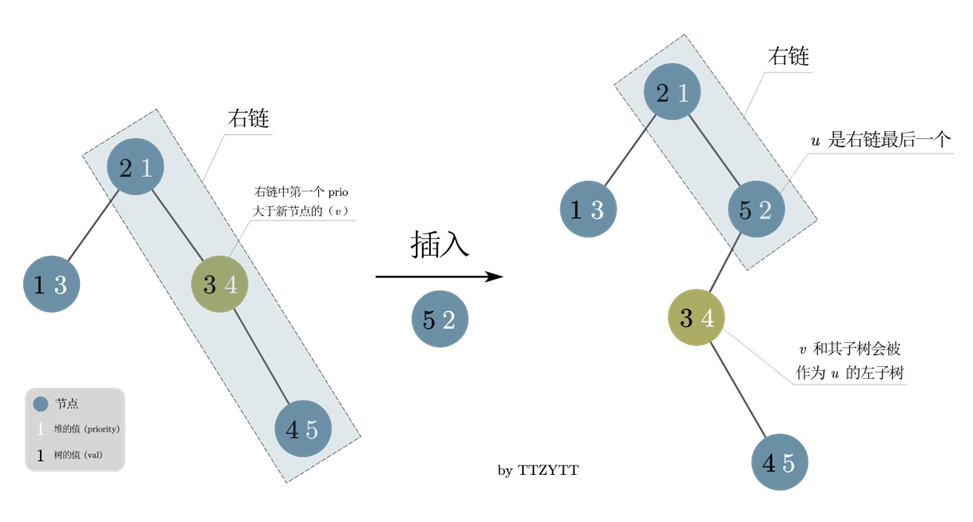
\includegraphics[width=\textwidth]{images/Treap_build.png}
        \end{figure}
    \end{frame}

    
    \begin{frame}
        \frametitle{单调栈建笛卡尔树}
        显然每个数最多进出右链一次(或者说每个点在右链中存在的是一段连续的时间)。这个过程可以用栈维护,栈中维护当前笛卡尔树的右链上的结点。一个点不在右链上了就把它弹掉。这样每个点最多进出一次,复杂度 $O(n)$。
    \end{frame}

    \subsection{时间复杂度}

    \begin{frame}
        \frametitle{时间复杂度}
        前面说过,二叉搜索树的操作的时间复杂度都是取决于树的深度。
        
        我们可以感性理解:
        Treap为了解决这个问题、达到一个较为「平衡」的状态,通过维护随机的优先级满足堆性质,「打乱」了结点的插入顺序,从而让二叉搜索树达到了理想的复杂度,避免了退化成链的问题。
        
        接下来我们开始证明时间复杂度:
        
        首先我们规定:排名为$i$的结点称为结点$i$,$A(x,y)$代表$x$是否$y$是的祖先,是则为$1$,不是则为$0$,$A(x,x)=0$,$\Pr(x)$代表$x$时间发生的概率,$E(x)$表示x的期望。

        单次操作$x$的时间复杂度为$x$的深度,而$x$的深度可以表示为祖先的数量:
        \[dep(x)=\sum_{i=1}^{n}A(i,x)\]
    \end{frame}

    \begin{frame}
        \frametitle{时间复杂度}
        \begin{tcolorbox}[colframe=blue,title=引理]
            \[A(x,y)=[priority_x=\min_{i=min(x,y)}^{max(x,y)}priority_i](x\neq y)\]
            证明:

            若$x$是$y$的祖先,$A(x,y)=1$,由小根堆的性质可知$priority_x$必定是最小的,所以$priority_x=\min_{i=min(x,y)}^{max(x,y)}priority_i$。

            若$y$是$x$的祖先,$A(x,y)=0$,由小根堆的性质可知$priority_y$必定是最小的,所以$priority_x\neq\min_{i=min(x,y)}^{max(x,y)}priority_i$。

            若$x$不是$y$的祖先,$y$也不是$x$的祖先,$A(x,y)=0$,$min(x,y)<LCA(x,y)<max(x,y)$,由小根堆的性质可知$priority_{LCA(x,y)}$必定是最小的,所以$priority_x\neq\min_{i=min(x,y)}^{max(x,y)}priority_i$。
        \end{tcolorbox}
    \end{frame}

    \begin{frame}
        \frametitle{时间复杂度}
        \[dep(x)=\sum_{i=1,i\neq x}^{n}[priority_i=\min_{j=min(i,x)}^{max(i,x)}priority_j]\]
        \[E(dep(x))=\sum_{i=1,i\neq x}^{n}E([priority_x=\min_{j=min(i,x)}^{max(i,x)}priority_j])\]
        \[E(dep(x))=\sum_{i=1,i\neq x}^{n}\Pr(priority_x=\min_{j=min(i,x)}^{max(i,x)}priority_j)\]
        因为$priority$是随机生成的,所以
        \[\Pr(priority_x=\min_{i=min(x,y)}^{max(x,y)}priority_i)=\frac{1}{\left\lvert x-y\right\rvert+1}\]    
        \[E(dep(x))=\sum_{i=1,i\neq x}^{n}\frac{1}{\left\lvert i-x\right\rvert+1}\]
    \end{frame}

    \begin{frame}
        \frametitle{时间复杂度}
        \begin{align}
            E(dep(x))&=\sum_{i=1}^{x-1}\frac{1}{x-i+1}+\sum_{i=x+1}^{n}\frac{1}{i-x+1}\nonumber\\
                     &=\sum_{i=2}^{x}\frac{1}{i}+\sum_{i=2}^{n-x+1}\frac{1}{i}\nonumber\\
                     &\le\sum_{i=2}^{n}\frac{1}{i}+\sum_{i=2}^{n}\frac{1}{i}\nonumber\\
                     &=2\sum_{i=2}^{n}\frac{1}{i}<2\sum_{i=2}^{n}\int_{i-1}^{i}\frac{1}{i}\,dx\nonumber\\
                     &=\int_{1}^{n}\frac{1}{i}\,dx=2\ln n=O(\log n)\nonumber
        \end{align}
        所以Treap的各操作时间复杂度都为$O(\log n)$
    \end{frame}

    \subsection{无旋Treap}

    \begin{frame}
        \frametitle{无旋Treap}
        无旋Treap,又称为FHQ Treap(范浩强),它维护堆的性质的方式与旋转Treap不同,它不需要旋转,而是通过分裂与合并来维护堆的性质。
    \end{frame}

    \begin{frame}
        \frametitle{分裂}
        分裂,指将Treap按照值大小或排名分列成两个树。
        分为按值分裂和按排名分裂。
        分裂同样通过递归实现。
    \end{frame}

    \begin{frame}[fragile]
        \frametitle{按值分裂}
        \begin{figure}
            \begin{minipage}[t]{0.4\textwidth}
                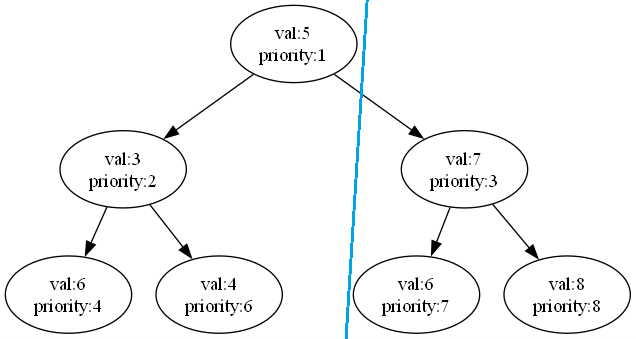
\includegraphics[height=0.8\linewidth]{images/Treap_split0.png}
                \caption{$val==cur\rightarrow val$}
            \end{minipage}
            \vfill
            \begin{minipage}[b]{0.4\textwidth}
                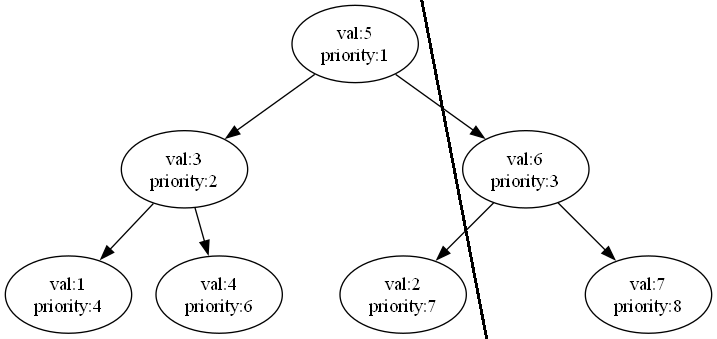
\includegraphics[width=\linewidth]{images/Treap_split1.png}
                \caption{$val>cur\rightarrow val$}
            \end{minipage}
            \hfill
            \begin{minipage}[b]{0.4\textwidth}
                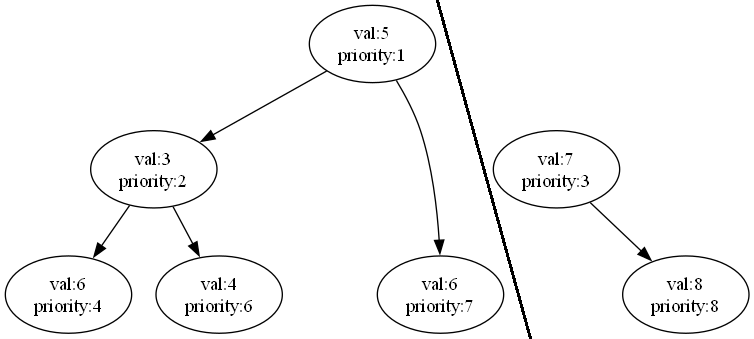
\includegraphics[width=\linewidth]{images/Treap_split2.png}
                \caption{$val>cur\rightarrow val$}
            \end{minipage}
        \end{figure}    
    \end{frame}

    \begin{frame}[fragile]
        \frametitle{按值分裂}
        \begin{lstlisting}[language=c++]
std::pair<Node*, Node*> split(Node *cur, int val) {
    if (!cur) return {nullptr, nullptr};
    if (!cmp(val, cur->val)) { // cur->val<=val,cur与cur左子树为左部分
#if (__cplusplus >= 201703L) // 分裂右子树为left和right
        auto [left, right] = split(cur->rightSon, val);
#elif
        Node *left, *right;
        std::tie(left, right) = split(cur->rightSon, val);
#endif // 将cur与右子树分裂后的左半部分连接
        cur->rightSon = left; 
        cur->update();
        return {cur, right};
    } else { // cur与cur右子树为右部分
#if (__cplusplus >= 201703L) // 分裂左子树为left和right
        auto [left, right] = split(cur->leftSon, val);
#elif
        Node *left, *right;
        std::tie(left, right) = split(cur->leftSon, val);
#endif // 将cur与左子树分裂后的右半部分连接
        cur->leftSon = right;
        cur->update();
        return {left, cur};
    }
}
        \end{lstlisting}
    \end{frame}

    \begin{frame}[fragile]
        \frametitle{按排名分裂}
        \begin{lstlisting}[language=c++]
std::tuple<Node*, Node*, Node*> splitByRank(Node *cur, size_t rank) {
    if (cur == nullptr) return {nullptr, nullptr, nullptr};
    size_t LeftSonSize = cur->leftSon ? cur->leftSon->size : 0;
    if (rank <= LeftSonSize) {
        Node *l, *mid, *r;
        std::tie(l, mid, r) = splitByRank(cur->leftSon, rank);
        cur->leftSon = r;
        cur->update();
        return {l, mid, cur};
    } else if (rank <= LeftSonSize + cur->cnt) {
        Node *l = cur->leftSon, *r = cur->rightSon;
        cur->leftSon = cur->rightSon = nullptr;
        return {l, cur, r};
    } else {
        Node *l, *mid, *r;
        std::tie(l, mid, r) = splitByRank(cur->rightSon, rank - LeftSonSize - cur->cnt);
        cur->rightSon = l;
        cur->update();
        return {cur, mid, r};
    }
}
        \end{lstlisting}
    \end{frame}
    
    \begin{frame}[fragile]
        \frametitle{合并}
        合并也是递归实现,在合并两棵树时,将$priority$较小的当做根。
        \begin{lstlisting}[language=c++]
Node *merge(Node *u, Node *v) {
    if (u == nullptr && v == nullptr) return nullptr;
    if (v == nullptr) return u;
    if (u == nullptr) return v;
    if (u->priority < v->priority) {
        v->leftSon = merge(u, v->leftSon);
        v->update();
        return v;
    } else {
        u->rightSon = merge(u->rightSon, v);
        u->update();
        return u;
    }
}
        \end{lstlisting}
    \end{frame}

    \begin{frame}[fragile]
        \frametitle{插入}
        先按插入值分为三部分:权值小于插入值、权值等于插入值、权值大于插入值。在将权值等于插入值的结点处理,再将三部分合并。
        \begin{lstlisting}[language=c++]
void insert(int val) {
    Node *left, *mid, *right;
    tie(left, right) = split(root, val);
    tie(left, mid) = split(left, val - 1);
    if (mid) {
        mid->cnt++, mid->size++;
    } else {
        mid = new Node(val);
    }
    root = merge(merge(left, mid), right);
}
        \end{lstlisting}
    \end{frame}
    
    \begin{frame}[fragile]
        \frametitle{删除}
        先按删除值分为三部分:权值小于删除值、权值等于删除值、权值大于删除值。在将权值等于删除值的结点处理,再将三部分合并。
        \begin{lstlisting}[language=c++]
void erase(int val) {
    Node *left, *mid, *right;
    tie(left, right) = split(root, val);
    tie(left, mid) = split(left, val - 1);
    if (mid) {
        if (mid->cnt > 1) {
            mid->cnt--, mid->size--;
        } else {
            delete mid;
            mid = nullptr;
        }
    }
    root = merge(merge(left, mid), right);
}
        \end{lstlisting}
    \end{frame}

    \begin{frame}[fragile]
        \frametitle{查询第K小}
        按排名K分裂为三部分,排名为K的结点的值即为答案。
        \begin{lstlisting}[language=c++]
size_t queryRank(Type val) {
    Node *l, *r;
    std::tie(l, r) = split(root, val - 1);
    size_t res = (l ? l->size : 0) + 1;
    root = merge(l, r);
    return res;
}
        \end{lstlisting}
    \end{frame}

    \begin{frame}[fragile]
        \frametitle{查询排名}
        按查询值分裂为两部分:权值小于查询值、权值大于等于查询值,左半部分大小加一即为排名。
        \begin{lstlisting}[language=c++]
Type queryKth(size_t rank) {
    if (rank > root->size) {
        throw NoSuchValueException("No so many vals in the treap");
    }
    Node *l, *mid, *r;
    std::tie(l, mid, r) = splitByRank(root, rank);
    root = merge(l, merge(mid, r));
    return mid->val;
}          
        \end{lstlisting}
    \end{frame}

    \begin{frame}[fragile]
        \frametitle{查询前驱}
        按查询值减一分裂为两部分,左部分最大的为前驱。
        \begin{lstlisting}[language=c++]
Type predecessor(Type val) {
    Node *l, *r;
    std::tie(l, r) = split(root, val - 1);
    if (l == nullptr) {
        root = merge(l, r);
        throw NoSuchValueException("No lower val in the treap");
        return Type();
    }
    Node *ll, *mid, *rr;
    std::tie(ll, mid, rr) = splitByRank(l, l->size);
    root = merge(merge(ll, mid), r);
    return mid->val;
}
        \end{lstlisting}
    \end{frame}

    \begin{frame}[fragile]
        \frametitle{查询后继}
        按查询值分裂为两部分,右部分最小的为后继。
        \begin{lstlisting}[language=c++]
Type successor(Type val) {
    Node *l, *r;
    std::tie(l, r) = split(root, val);
    if (r == nullptr) {
        root = merge(l, r);
        throw NoSuchValueException("No higher val in the treap");
        return Type();
    }
    Node *ll, *mid, *rr;
    std::tie(ll, mid, rr) = splitByRank(r, 1);
    root = merge(l, merge(mid, rr));
    return mid->val;
}
        \end{lstlisting}
    \end{frame}

    \begin{frame}
        \frametitle{建树}
        我们可以二分递归建树,建完左子树和右子树,将左子树、根、右子树合并起来就可以了。这样建树的时间复杂度是$O(n)$的。
        
        证明:每个点都需要合并一次,合并的时间复杂度取决于左右子树的深度。假如这个点深度为$i$,则他的子树的深度不超过$\left\lceil\log n\right\rceil-i$,因为第$i$层有$2^{i-1}$个节点,所以总时间复杂度为:
        \begin{align}
             &\sum_{i=1}^{\left\lceil\log n\right\rceil}2^{i-1}(\left\lceil\log n\right\rceil-i)\nonumber\\
            =&\sum_{i=1}^{\left\lceil\log n\right\rceil}(2^{i-1}\left\lceil\log n\right\rceil-2^{i-1}\cdot i)\nonumber\\
            =&\sum_{i=1}^{\left\lceil\log n\right\rceil}2^{i-1}\left\lceil\log n\right\rceil-\sum_{i=1}^{\left\lceil\log n\right\rceil}2^{i-1}\cdot i\nonumber\\
            =&\left\lceil\log n\right\rceil\sum_{i=0}^{\left\lceil\log n\right\rceil-1}2^i-\sum_{i=1}^{\left\lceil\log n\right\rceil}2^{i-1}\cdot i\nonumber
        \end{align}
    \end{frame}

    \begin{frame}
        \frametitle{建树}
        \tiny
        \begin{align}
              =&\left\lceil\log n\right\rceil\sum_{i=0}^{\left\lceil\log n\right\rceil-1}2^i-\sum_{i=1}^{\left\lceil\log n\right\rceil}2^{i-1}\cdot i\nonumber\\
              =&\left\lceil\log n\right\rceil(2^{\left\lceil\log n\right\rceil}-1)-\sum_{i=1}^{\left\lceil\log n\right\rceil}2^{i-1}\cdot i\nonumber\\
            \le&\left\lceil\log n\right\rceil(2n-1)-\sum_{i=1}^{\left\lceil\log n\right\rceil}2^{i-1}\cdot i\nonumber\\
              =&\left\lceil\log n\right\rceil(2n-1)-(\sum_{i=1}^{\left\lceil\log n\right\rceil}2^{i}\cdot i-\sum_{i=1}^{\left\lceil\log n\right\rceil}2^{i-1}\cdot i)\nonumber\\
              =&\left\lceil\log n\right\rceil(2n-1)-(\sum_{i=0}^{\left\lceil\log n\right\rceil}2^{i}\cdot i-\sum_{i=0}^{\left\lceil\log n\right\rceil-1}2^i\cdot (i+1))\nonumber\\
              =&\left\lceil\log n\right\rceil(2n-1)-(2^{\left\lceil\log n\right\rceil}\cdot \left\lceil\log n\right\rceil+\sum_{i=0}^{\left\lceil\log n\right\rceil-1}2^{i}\cdot i-\sum_{i=0}^{\left\lceil\log n\right\rceil-1}2^i\cdot (i+1))\nonumber\\
              =&\left\lceil\log n\right\rceil(2n-1)-(2^{\left\lceil\log n\right\rceil}\cdot \left\lceil\log n\right\rceil-\sum_{i=0}^{\left\lceil\log n\right\rceil-1}2^{i}\nonumber\\
              =&\left\lceil\log n\right\rceil(2n-1)-(2^{\left\lceil\log n\right\rceil}\cdot \left\lceil\log n\right\rceil-(2^{\left\lceil\log n\right\rceil}-1))\nonumber\\
            \le&\left\lceil\log n\right\rceil(2n-1)-2n\cdot \left\lceil\log n\right\rceil+2n-1\nonumber\\
            \le&\left\lceil\log n\right\rceil(2n-1)-2n\cdot \left\lceil\log n\right\rceil+2n-1\nonumber\\
              =&-\left\lceil\log n\right\rceil+2n-1<2n=O(n)\nonumber
        \end{align}
    \end{frame}

    \subsection{区间操作}

    \begin{frame}
        \frametitle{无旋Treap的区间操作}
        一些平衡树可以像线段树一样支持区间操作,也同样可以和线段树一样打懒标记,而且功能比线段树更多,比如可以区间翻转操作,但常数可能略高。

        在维护区间操作时,树并不需要满足BST的性质。为了维护区间操作,平衡树往往需要将某个区间提取出来。

        而无旋Treap通过分裂把需要操作的区间分裂出来,然后打上懒标记,合并起来。
    \end{frame}

    \begin{frame}
        \frametitle{\href{https://www.luogu.com.cn/problem/P3391}{P3391 【模板】文艺平衡树}}
        \framesubtitle{\textcolor[RGB]{52, 152, 219}{提高+/省选−}}        
        【题目描述】

        您需要写一种数据结构(可参考题目标题),来维护一个有序数列。  

        其中需要提供以下操作:翻转一个区间,例如原有序序列是 $5\ 4\ 3\ 2\ 1$,翻转区间是 $[2,4]$ 的话,结果是 $5\ 2\ 3\ 4\ 1$。

        【数据范围】  

        对于 $100\%$ 的数据,$1 \le n, m \leq 100000 $,$1 \le l \le r \le n$。
    \end{frame}

    \begin{frame}
        \frametitle{无旋Treap}
        先建树,每一次操作分裂出区间,把分裂出的根上打上懒标记。注意分裂合并的时候下传标记。    
    \end{frame}

    \begin{frame}
        \frametitle{\href{https://www.luogu.com.cn/problem/P2042}{P2042 [NOI2005] 维护数列}}
        \framesubtitle{\textcolor[RGB]{157,61,207}{省选/NOI−}}
        请写一个程序,要求维护一个数列,支持以下 $6$ 种操作:

        \begin{table}[h]
            \tiny
            \centering
            \begin{tabularx}{\textwidth}{|c|c|c|X|}
                \hline
                编号 & 名称 & 格式 & 说明 \\ \hline
                1 & 插入 & $\operatorname{INSERT}\ posi \ tot \ c_1 \ c_2 \cdots c_{tot}$ & 在当前数列的第 $posi$ 个数字后插入 $tot$ 个数字:$c_1, c_2 \cdots c_{tot}$;若在数列首插入,则 $posi$ 为 $0$ \\ \hline
                2 & 删除 & $\operatorname{DELETE} \ posi \ tot$ & 从当前数列的第 $posi$ 个数字开始连续删除 $tot$ 个数字 \\ \hline
                3 & 修改 & $\operatorname{MAKE-SAME} \ posi \ tot \ c$ & 从当前数列的第 $posi$ 个数字开始的连续 $tot$ 个数字统一修改为 $c$ \\ \hline
                4 & 翻转 & $\operatorname{REVERSE}\ posi \ tot$ & 取出从当前数列的第 $posi$ 个数字开始的 $tot$ 个数字,翻转后放入原来的位置 \\ \hline
                5 & 求和 & $\operatorname{GET-SUM} \ posi \ tot$ & 计算从当前数列的第 $posi$ 个数字开始的 $tot$ 个数字的和并输出 \\ \hline
                6 & 求最大子列和 & $\operatorname{MAX-SUM}$ & 求出当前数列中和最大的一段子列,并输出最大和 \\ \hline
            \end{tabularx}
        \end{table}
        数据规模与约定

        - 对于 $50\%$ 的数据,任何时刻数列中最多含有 $3 \times 10^4$ 个数。

        - 对于 $100\%$ 的数据,任何时刻数列中最多含有 $5 \times 10^5$ 个数,任何时刻数列中任何一个数字均在 $[-10^3, 10^3]$ 内,$1 \le M \le 2 \times 10^4$,插入的数字总数不超过 $4 \times 10^6$。
    \end{frame}

    \begin{frame}
        \frametitle{\href{https://www.luogu.com.cn/problem/P2042}{P2042 [NOI2005] 维护数列}}
        \framesubtitle{\textcolor[RGB]{157,61,207}{省选/NOI−}}
        这道题目与文艺平衡树类似,但是操作更加的复杂,我们在处理懒标记时也要更加注意。

        因为题目要求维护最大子段和,我们可以仿照线段树例题\href{https://www.luogu.com.cn/problem/P4513}{P4513 小白逛公园},对于一个区间,我们维护最大子段和,从左端点起的最大子段和,从右端点结束的最大子段和以及区间的总和。

        注:
        \begin{itemize}
            \item 这题不用指针随时释放空间的话会MLE,需要模拟内存/指针实现。
            \item 题面中$tot$可能为$0$,不特判有可能使你的代码RE80pts。
            \item 要仔细处理update函数。
        \end{itemize}
        
    \end{frame}

    \section{Splay}

    \begin{frame}
        \frametitle{Splay}
        Splay(伸展)也是一种平衡树,它通过Splay操作使树平衡。

        Splay 树由 Daniel Sleator 和 Robert Tarjan 于 1985 年发明。

        Splay树每次操作都通过Splay操作需要将结点旋转到根。 
    \end{frame}

    \subsection{操作}

    \begin{frame}
        \frametitle{Splay操作}
        Splay/伸展操作,指将某个结点旋转到根的操作。

        Splay操作的步骤分为6种,zig、zig-zig、zig-zag、zag、zag-zag、zag-zig。这里我们主要介绍前三种,因为后三种就是前三种左右对称的。  
    \end{frame}

    \begin{frame}[fragile]
        \frametitle{旋转}
        Splay操作是基于旋转的,而Splay的旋转略有不同。
        \begin{figure}
            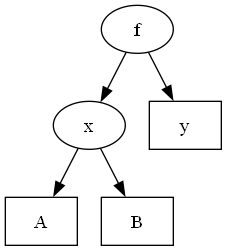
\includegraphics[width=0.3\textwidth]{images/right_rotate0.png}
            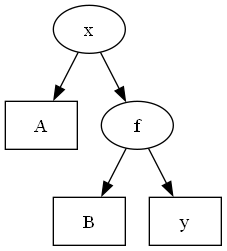
\includegraphics[width=0.3\textwidth]{images/right_rotate2.png}
        \end{figure}
        我们说旋转$x$结点,指的是将$x$旋转的其父结点,而不是将$x$的子结点旋转到$x$,而且要我们还要维护父节点。
        \begin{lstlisting}[language=c++]
void rotate(Node *&cur) {
    Node *father = cur->father;
    Node *grandfather = father->father;
        \end{lstlisting}
    \end{frame}

    \begin{frame}[fragile]
        \frametitle{旋转}
        \begin{lstlisting}[language=c++]
    if (grandfather) {
        if (father->isLeftSon()) {
            grandfather->leftSon = cur;
        } else {
            grandfather->rightSon = cur;
        }
    }
    if (cur->isLeftSon()) {
        father->leftSon = cur->rightSon;
        if (father->leftSon) {
            father->leftSon->father = father;
        }
        cur->rightSon = father;
    } else {
        father->rightSon = cur->leftSon;
        if (father->rightSon) {
            father->rightSon->father = father;
        }
        cur->leftSon = father;
    }
    cur->father = grandfather;
    father->father = cur;
    father->update();
    cur->update();
}
        \end{lstlisting}
    \end{frame}

    \begin{frame}
        \frametitle{zig操作}
        \begin{figure}
            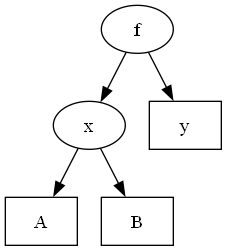
\includegraphics[width=0.3\textwidth]{images/right_rotate0.png}
            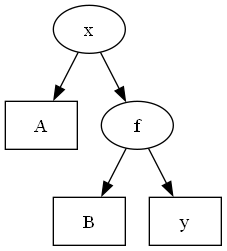
\includegraphics[width=0.3\textwidth]{images/right_rotate2.png}
        \end{figure}
        zig和zag操作当且仅当在$x$的父结点$f$是树的根结点时执行,具体来说就是旋转$x$结点。
    \end{frame}

    \begin{frame}
        \frametitle{zig-zig操作}
        \begin{figure}
            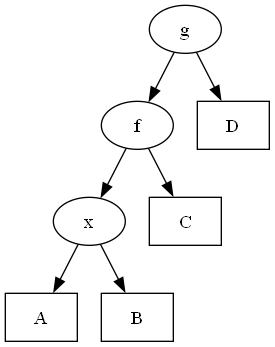
\includegraphics[width=0.25\textwidth]{images/splay_zig-zig0.png}
            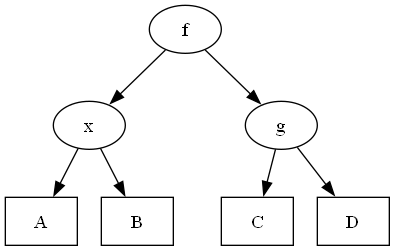
\includegraphics[width=0.4\textwidth]{images/splay_zig-zig1.png}
            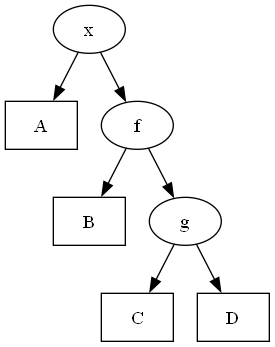
\includegraphics[width=0.25\textwidth]{images/splay_zig-zig2.png}
        \end{figure}
        zig-zig和zag-zag操作在$f$的子结点$x$和$g$结点的子结点$f$在同侧时执行,具体来说是先旋转$f$结点,在旋转$x$结点。
    \end{frame}

    \begin{frame}
        \frametitle{zig-zag操作}
        \begin{figure}
            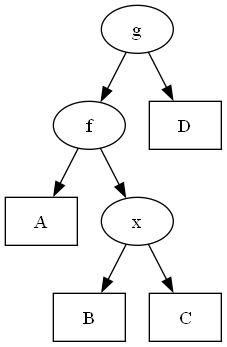
\includegraphics[width=0.25\textwidth]{images/splay_zig-zag0.png}
            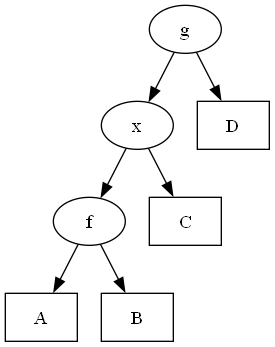
\includegraphics[width=0.3\textwidth]{images/splay_zig-zag1.png}
            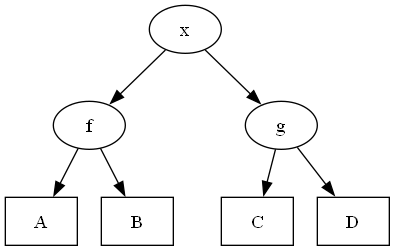
\includegraphics[width=0.4\textwidth]{images/splay_zig-zag2.png}
        \end{figure}
        zig-zag和zag-zig操作在$f$的子结点$x$和$g$结点的子结点$f$在异侧时执行,具体来说是先旋转一次$x$结点,在旋转一次$x$结点。
    \end{frame}

    \begin{frame}[fragile]
        \frametitle{Splay操作}
        综上所述,我们发现无论是这六种操作的哪一种最后都需要旋转$x$结点,而先旋转哪个结点,取决于$x$和$f$是否同侧。
        \begin{lstlisting}[language=c++]
Node* splay(Node *cur) {
    for (Node *fa; fa = cur->father;) {
        if (fa->father) {
            rotate(cur->isLeftSon() == fa->isLeftSon() ? fa : cur);
        }
        rotate(cur);
    }
    return root = cur;
}       
        \end{lstlisting}
    \end{frame}
    
    \begin{frame}[fragile]
        \frametitle{插入}
        Splay的插入操作只需要注意在插入后不要忘记Splay操作。
        \begin{lstlisting}[language=c++]
void _insert(Node *&cur, Type val, Node *father = nullptr) {
    if (!cur) {
        cur = new Node(val, father);
        if (father) father->update();
        splay(cur);
        return;
    }
    if (cur->val == val) {
        cur->cnt++;
        cur->update();
        splay(cur);
    } else if (cmp(val, cur->val)){
        _insert(cur->leftSon, val, cur);
    } else {
        _insert(cur->rightSon, val, cur);
    }
}
        \end{lstlisting}
    \end{frame}

    \begin{frame}[fragile]
        \frametitle{删除}

        首先找到$val$等于删除值的$x$结点,然后将$x$结点旋转到根,如果$x$结点的$cnt$大于$1$,那么直接将$cnt$减$1$即可,但如果$cnt=1$,那么我们就需要合并$x$的左右子树。
        \begin{tcolorbox}[colframe=blue,title=合并子树]
            如果两棵子树都为空,合并后也为空

            如果其中一个为空,返回另一个。

            如果两个都不为空,将左子树的最大值旋转到左子树的根,将左子树的根的右子树设为要合并的右子树。(这里选取右子树的最小值旋转到根也是同理)
        \end{tcolorbox}
        \begin{lstlisting}[language=c++]
bool erase(Type val) {
    Node *cur = find(val);
    if (cur == nullptr) return false;
    if (cur->cnt > 1) {
        cur->cnt--;
        cur->update();
        return true;
    }
        \end{lstlisting}
    \end{frame}

    \begin{frame}[fragile]
        \frametitle{删除}
        \begin{lstlisting}[language=c++]            
    if (!cur->leftSon && !cur->rightSon) {
        delete cur;
        root = nullptr;
    } else if (!cur->leftSon) {
        root = cur->rightSon;
        root->father = nullptr;
    } else if (!cur->rightSon) {
        root = cur->leftSon;
        root->father = nullptr;
    } else {
        cur->leftSon->father = nullptr;
        splay(_predecessor());
        root->rightSon = cur->rightSon;
        if (cur->rightSon) cur->rightSon->father = root;
        delete cur;
    }
    return true;
}
        \end{lstlisting}    
    \end{frame}

    \begin{frame}[fragile]
        \frametitle{查询排名}
        找到$x$结点后,将$x$旋转到根,左子树的大小加一即为排名。
        \begin{lstlisting}[language=c++]
int queryRank(Type val) {
    _insert(root, val);
    int res = root->leftSon ? root->leftSon->size + 1 : 1;
    erase(val);
    return res;
}
        \end{lstlisting}
    \end{frame}

    \begin{frame}[fragile]
        \frametitle{查询第K小}
        \begin{lstlisting}[language=c++]
Type _queryKth(Node *&cur, int rank) {
    int leftSonSize = cur->leftSon ? cur->leftSon->size : 0;
    if (rank <= leftSonSize) {
        return _queryKth(cur->leftSon, rank);
    } else if (rank <= leftSonSize + cur->cnt) {
        return splay(cur)->val;
    } else if (rank <= cur->size) {
        return _queryKth(cur->rightSon, rank - leftSonSize - cur->cnt);
    }
}
        \end{lstlisting}    
    \end{frame}

    \begin{frame}[fragile]
        \frametitle{查询前驱}
        模版中查询前驱并不保证$x$在集合中,所以我们需要先将$x$插入到集合中,此时$x$已经在根的位置,查询左子树最大值即可,具体来说就是从左子树的根一直向右,最后到达的就是左子树中的最大值。
        \begin{lstlisting}[language=c++]
Node *_predecessor() {
    Node *cur = root->leftSon;
    if (!cur) return nullptr;
    while (cur->rightSon) {
        cur = cur->rightSon;
    }
    return splay(cur);
}
        \end{lstlisting}
    \end{frame}

    \begin{frame}[fragile]
        \frametitle{查询后继}
        查询后继与查询前驱类似,找右子树的最小值。
        \begin{lstlisting}[language=c++]
Node *_successer() {
    Node *cur = root->rightSon;
    if (!cur) return nullptr;
    while (cur->leftSon) {
        cur = cur->leftSon;
    }
    return splay(cur);
}
        \end{lstlisting}
    \end{frame}

    \subsection{时间复杂度}

    \begin{frame}
        \frametitle{时间复杂度}
        Splay树的各个操作都是基于Splay操作的,所以我们只需要分析Splay操作的时间复杂度。

        Splay操作有6种,但zig和zag是对称的,我们只分析zig、zig-zig、zig-zag。

        这里我们先引进势能分析法。
    \end{frame}

    \begin{frame}
        \frametitle{势能分析法}
        势能分析法是摊还分析的一种,借用了物理学中的概念,还分析将数据结构中的预付代价表示为“势能”,将积攒的势能释放可以支付未来操作的代价,将势能与整个数据结构相关联。
        
        对于一个初始数据结构$D_0$,此时数据结构的势能为$\Phi(D_0)$,我们有$m$次操作,第$i$次操作后数据结构变为$D_i$,此时数据结构的势能为$\Phi(D_i)$

        势能分析法将第$i$次操作的均摊成本设为:$\hat{c_i}=c_i+\Phi(D_i)-\Phi(D_{i-1})$,其中$c_i$为实际的代价。
    \end{frame}

    \begin{frame}
        \frametitle{势能分析法}
        若一共有$m$次操作,则总的均摊成本为:
        \begin{align}
            \sum_{i=1}^m\hat{c_i}&=\sum_{i=1}^m(c_i+\Phi(D_i)-\Phi(D_{i-1}))\nonumber\\
                                 &=\sum_{i=1}^mc_i+\sum_{i=1}^m\Phi(D_i)-\sum_{i=1}^m\Phi(D_{i-1})\nonumber\\
                                 &=\sum_{i=1}^mc_i+\Phi(D_m)+\sum_{i=1}^{m-1}\Phi(D_i)-\sum_{i=0}^{m-1}\Phi(D_i)\nonumber\\
                                 &=\sum_{i=1}^mc_i+\Phi(D_m)-\Phi(D_0)\nonumber
        \end{align}
        总的实际的时间复杂度就是$\sum_{i=1}^m\hat{c_i}+\Phi(D_0)-\Phi(D_m)$
    \end{frame}

    \begin{frame}
        \frametitle{Splay}
        设结点$x$的势能为:$\phi(x)=\log\left\lvert x\right\rvert$,$\left\lvert x\right\rvert$为$x$结点的子树大小。

        性质:如果$\left\lvert z\right\rvert\ge\left\lvert x\right\rvert+\left\lvert y\right\rvert$,则$2\phi(z)-\phi(x)-\phi(y)\ge2$
        
        证明:
        \begin{align}
            2\phi(z)-\phi(x)-\phi(y)&=2\log\left\lvert z\right\rvert-\log\left\lvert x\right\rvert-\log\left\lvert y\right\rvert\nonumber\\
                                    &=\log\frac{\left\lvert z\right\rvert^2}{\left\lvert x\right\rvert\cdot\left\lvert y\right\rvert}\nonumber\\
                                    &\ge\log\frac{(\left\lvert x\right\rvert+\left\lvert y\right\rvert)^2}{\left\lvert x\right\rvert\cdot\left\lvert y\right\rvert}\nonumber\\
                                    &\ge\log\frac{\left\lvert x\right\rvert^2+\left\lvert y\right\rvert^2+2\left\lvert x\right\rvert\cdot\left\lvert y\right\rvert}{\left\lvert x\right\rvert\cdot\left\lvert y\right\rvert}\nonumber\\
                                    &\ge\log\frac{4\left\lvert x\right\rvert\cdot\left\lvert y\right\rvert}{\left\lvert x\right\rvert\cdot\left\lvert y\right\rvert}\ge\log4\ge2\nonumber
        \end{align}
        设整棵树的势能$\Phi=\sum \phi(x)$
        
        我们先把Splay操作分成各个小操作,设每个小操作的均摊成本为$\hat{c'_i}=c'_i+\Phi(D')-\Phi(D)$
        我们将$\phi'(x)$设为$x$移动后的势能
    \end{frame}

    \begin{frame}
        \frametitle{zig操作}
        \begin{figure}
            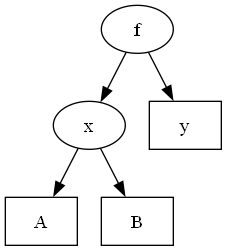
\includegraphics[width=0.3\textwidth]{images/right_rotate0.png}
            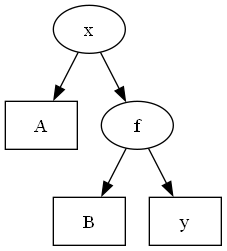
\includegraphics[width=0.3\textwidth]{images/right_rotate2.png}
        \end{figure}
        \begin{align}
            \hat{c'_i}&=1+\Phi(D')-\Phi(D)\nonumber\\
                      &=1+\phi'(x)+\phi'(f)-\phi(x)-\phi(f)\nonumber\\
                      &=1+\phi'(f)-\phi(x)\nonumber\\
                      &\le1+\phi'(x)-\phi(x)\nonumber
        \end{align}
    \end{frame}

    \begin{frame}
        \frametitle{zig-zig操作}
        \begin{figure}
            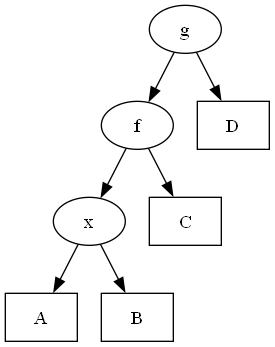
\includegraphics[width=0.25\textwidth]{images/splay_zig-zig0.png}
            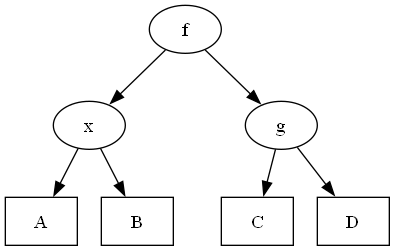
\includegraphics[width=0.4\textwidth]{images/splay_zig-zig1.png}
            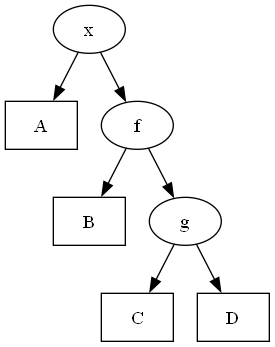
\includegraphics[width=0.25\textwidth]{images/splay_zig-zig2.png}
        \end{figure}
        \begin{align}
            \hat{c'_i}&=2+\Phi(D')-\Phi(D)\nonumber\\
                      &=2+\phi'(x)+\phi'(f)+\phi'(g)-\phi(x)-\phi(f)-\phi(g)\nonumber\\
                      &=2+\phi'(f)+\phi'(g)-\phi(x)-\phi(f)\nonumber
        \end{align}
        \[\because\left\lvert x'\right\rvert=\left\lvert A\right\rvert+\left\lvert B\right\rvert+\left\lvert C\right\rvert+\left\lvert D\right\rvert+3,\left\lvert x\right\rvert=\left\lvert A\right\rvert+\left\lvert B\right\rvert+1,\left\lvert g'\right\rvert=\left\lvert C\right\rvert+\left\lvert D\right\rvert+1\]
        \[\because\left\lvert x'\right\rvert>\left\lvert x\right\rvert+\left\lvert g'\right\rvert\]
        \[\therefore2\phi'(x)-\phi(x)-\phi'(g)\ge2\]
        \[\hat{c'_i}\le2\phi'(x)-\phi(x)-\phi'(g)+\phi'(f)+\phi'(g)-\phi(x)-\phi(f)\]
    \end{frame}

    \begin{frame}
        \frametitle{zig-zig操作}
        \begin{align}
            \hat{c'_i}&\le2\phi'(x)-\phi(x)-\phi'(g)+\phi'(f)+\phi'(g)-\phi(x)-\phi(f)\nonumber\\
                      &=2\phi'(x)-2\phi(x)+\phi'(f)-\phi(f)\nonumber\\
                      &\le2\phi'(x)-2\phi(x)+\phi'(x)-\phi(x)\nonumber\\
                      &=3(\phi'(x)-\phi(x))\nonumber
        \end{align}
    \end{frame}

    \begin{frame}
        \frametitle{zig-zag操作}
        \begin{figure}
            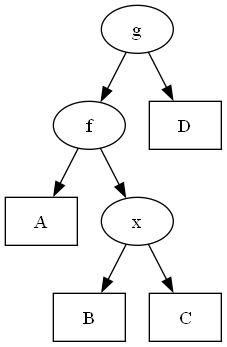
\includegraphics[width=0.25\textwidth]{images/splay_zig-zag0.png}
            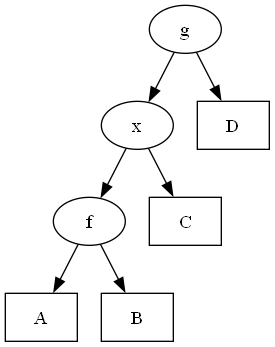
\includegraphics[width=0.3\textwidth]{images/splay_zig-zag1.png}
            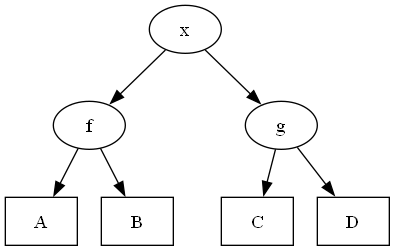
\includegraphics[width=0.4\textwidth]{images/splay_zig-zag2.png}
        \end{figure}
        \begin{align}
            \hat{c'_i}&=2+\Phi(D')-\Phi(D)\nonumber\\
                      &=2+\phi'(x)+\phi'(f)+\phi'(g)-\phi(x)-\phi(f)-\phi(g)\nonumber\\
                      &=2+\phi'(f)+\phi'(g)-\phi(x)-\phi(f)\nonumber
        \end{align}
        \[\because\left\lvert x\right\rvert=\left\lvert f\right\rvert+\left\lvert g\right\rvert+1\]
        \[\therefore\left\lvert x\right\rvert>\left\lvert f\right\rvert+\left\lvert g\right\rvert\]
        \[\therefore2\le2\phi'(x)-\phi'(f)-\phi'(g)\]
    \end{frame}

    \begin{frame}
        \frametitle{zig-zag操作}
        \begin{align}
            \hat{c'_i}&\le2\phi'(x)-\phi'(f)-\phi'(g)+\phi'(f)+\phi'(g)-\phi(x)-\phi(f)\nonumber\\
                      &=2\phi'(x)-\phi(x)-\phi(f)\nonumber\\
                      &\le2\phi'(x)-\phi(x)-\phi(x)\nonumber\\
                      &\le2(\phi'(x)-\phi(x))\nonumber\\
                      &\le3(\phi'(x)-\phi(x))\nonumber
        \end{align}
    \end{frame}

    \begin{frame}
        \frametitle{总结}
        因为zig操作可以放缩为$\le3(\phi'(x)-\phi(x))+1$,但至多执行一次,其余操作均能放缩为$\le3(\phi'(x)-\phi(x))$。
        所以
        \begin{align}
            \sum_{i=1}^{k}\hat{c'_i}&=1+\sum_{i=1}^{k}3(\phi^{(i)}(x)-\phi^{(i-1)}(x))\nonumber\\
                                    &=1+3\phi^{(k)}(x)-3\phi^{(0)}(x)\nonumber\\
                                    &=1+3\phi(root)-3\phi(x)\nonumber\\
                                    &\le1+\phi(root)\le1+3\log n\le O(\log n)\nonumber
        \end{align}
        \[\therefore\hat{c_i}=O(\log n)\]
        实际时间复杂度为$\sum_{i=1}^m\hat{c_i}+\Phi(D_0)-\Phi(D_m)$
            
        若结束时Splay中的节点全部被删除了,此时$\Phi(D_m)=0$

        若初始时Splay中有$n$个节点\[\Phi(D_0)=\sum_{i=1}^{n}\phi(i)\le\sum_{i=1}^{n}\log\left\lvert i\right\rvert\le\sum_{i=1}^{n}\log n=n\log n\]
    \end{frame}

    \begin{frame}
        \frametitle{总结}
        \begin{align}
            &\sum_{i=1}^m\hat{c_i}+\Phi(D_0)-\Phi(D_m)\nonumber\\
            \le&m\log n+n\log n-0\nonumber\\
            =&(n+m)\log n\nonumber
        \end{align}
        所以,Splay树的总时间复杂度为$O((n+m)\log n)$,每次splay操作和其它各的平均复杂度为$O(\log n)$。    
    \end{frame}

    \subsection{例题}

    \begin{frame}
        \frametitle{\href{https://www.luogu.com.cn/problem/P2596}{P2596 [ZJOI2006] 书架}}
        \framesubtitle{\textcolor[RGB]{157,61,207}{省选/NOI−}}
        \tiny
        第一行有两个整数,分别表示书的个数 $n$ 以及命令条数 $m$。

        第二行有 $n$ 个整数,第 $i$ 个整数表示初始时从上向下书第 $i$ 本书的编号 $p_i$。

        接下来 $m$ 行,每行表示一个操作。每行初始时有一个字符串  $op$。

        \begin{itemize}
            \item 若 $op$ 为 `Top`,则后有一个整数 $s$,表示把编号为 $s$ 的书放在最上面。
            \item 若 $op$ 为 `Bottom`,则后有一个整数 $s$,表示把编号为 $s$ 的书放在最下面。
            \item 若 $op$ 为 `Insert`,则后有两个整数 $s, t$,表示若编号为 $s$ 的书上面有 $x$ 本书,则放回这本书时他的上面有 $x + t$ 本书。
            \item 若 $op$ 为 `Ask`,则后面有一个整数 $s$,表示询问编号为 $s$ 的书上面有几本书。
            \item 若 $op$ 为 `Query`,则后面有一个整数 $s$,询问从上面起第 $s$ 本书的编号。
        \end{itemize}

        题目描述节选

        小 T 的记忆力是非常好的,所以每次放书的时候至少能够将那本书放在拿出来时的位置附近,比如说她拿的时候这本书上面有 $x$ 本书,那么放回去时这本书上面就只可能有 $x-1$、$x$ 或 $x+1$ 本书。

        数据规模与约定

        对于 $100\%$ 的数据,保证:$3 \leq n, m \leq 8 \times 10^4$,$p_i$ 是一个 $1 \sim n$ 的排列,$1 \leq s \leq n$,$-1 \leq t \leq 1$
    \end{frame}

    \begin{frame}
        \frametitle{\href{https://www.luogu.com.cn/problem/P2596}{P2596 [ZJOI2006] 书架}}
        \framesubtitle{\textcolor[RGB]{157,61,207}{省选/NOI−}}
        Splay,支持五个操作:
        \begin{enumerate}
            \item 将某元素置顶:将元素旋到根,然后将左子树合并到该元素的后继
            \item 将某元素置底:将元素旋到根,然后将右子树合并到该元素的前驱
            \item 将某元素提前/滞后1位:直接与该元素的前驱/后继交换位置及信息
            \item 询问指定元素排名:splay基本操作
            \item 询问指定排名元素:splay基本操作
        \end{enumerate}
        但是我们需要快速的找到编号对应的节点,就需要一个Map数组。
        操作的时候一定要仔细分析。
    \end{frame}

    \begin{frame}[fragile]
        \frametitle{代码}
        \begin{lstlisting}[language=c++]
Node *root, *Map[100000];
int p[100000], n, m;
Node *build(int p[], int l, int r, Node *fa = nullptr) {
    if (l > r) return nullptr;
    int mid = l + r >> 1;
    Node *t = new Node(p[mid], fa);
    t->leftSon = build(p, l, mid - 1, t);
    t->rightSon = build(p, mid + 1, r, t);
    t->update();
    return Map[p[mid]] = t;
}
Node *pre() {
    Node *x = root->leftSon;
    while (x->rightSon) x = x->rightSon;
    return x;
}
Node *suc() {
    Node *x = root->rightSon;
    while (x->leftSon) x = x->leftSon;
    return x;
}
        \end{lstlisting}
    \end{frame}

    \begin{frame}[fragile]
        \begin{lstlisting}[language=c++]
void top(int s) {
    root = splay(Map[s]);
    if (!root->leftSon) return;
    if (!root->rightSon) {
        root->rightSon = root->leftSon;
        root->leftSon = nullptr;
        return; 
    }
    root->rightSon->father = nullptr;
    root->rightSon = splay(suc());
    root->rightSon->father = root;
    swap(root->leftSon, root->rightSon->leftSon);
    root->rightSon->leftSon->father = root->rightSon;
    root->rightSon->update();
    root->update();
}
        \end{lstlisting}
    \end{frame}

    \begin{frame}[fragile]
        \frametitle{代码}
        \begin{lstlisting}[language=c++]
void insert(int s, int t) {
    if (!t) return;
    root = splay(Map[s]);
    Node *x = (t == 1 ? suc() : pre());
    if (x->father) {
        if (x->isLeftSon()) {
            x->father->leftSon = root;
        } else {
            x->father->rightSon = root;
        }
    }
    swap(root->leftSon, x->leftSon);
    swap(root->rightSon, x->rightSon);
    swap(root->father, x->father);
    if (root->leftSon) root->leftSon->father = root;
    if (root->rightSon) root->rightSon->father = root;
    if (x->leftSon) x->leftSon->father = x;
    if (x->rightSon) x->rightSon->father = x;
    root = splay(root);
}
int Ask(int s) {
    root = splay(Map[s]);
    return root->leftSon ? root->leftSon->size : 0;
}
        \end{lstlisting}
    \end{frame}

    \subsection{区间操作}

    \begin{frame}
        \frametitle{区间操作}
        由旋转的性质可知,Splay操作并不影响树的中序遍历。
        
        但是区间操作还需要将某段区间分离出来,Splay怎么实现呢?

        要想找到$[l,r]$这段区间,我们先将$l-1$通过Splay操作旋转到根,然后将$r+1$结点通过Splay操作旋转到根的右儿子,此时根的右子树的左子树即为区间$[l,r]$。

        但是假如$l=1$或者$r=n$时,在特殊处理就不太方便,所以我们在建树的时候会加上两个“哨兵”节点,就不再需要特殊处理。
    \end{frame}

    \begin{frame}[fragile]
        \frametitle{\href{https://www.luogu.com.cn/problem/P3391}{P3391 【模板】文艺平衡树}}
        \framesubtitle{\textcolor[RGB]{52, 152, 219}{提高+/省选−}}
        \begin{lstlisting}[language=c++]
struct Node {
    ...
    void addTag() {
        tag = !tag;
        swap(leftSon, rightSon);
    }
    void pushDown() {
        if (!tag) return;
        if (leftSon) leftSon->addTag();
        if (rightSon) rightSon->addTag();
        tag = 0;
    }
};
void splay2(Node *cur) {
    for (Node *fa; fa = cur->father, cur->father != root;) {
        if (fa->father != root) {
            rotate(fa->isLeftSon() == cur->isLeftSon() ? fa : cur);
        }
        rotate(cur);
    }
}

        \end{lstlisting}    
    \end{frame}
    
    \begin{frame}[fragile]
        \frametitle{代码}
        \begin{lstlisting}[language=c++]
void print(Node *cur = root) {
    if (!cur) return;
    cur->pushDown();
    print(cur->leftSon);
    if (cur->val > 0 && cur->val <= n)
        cout << cur->val << ' ';
    print(cur->rightSon);
}
int main() {
    scanf("%d%d", &n, &m);
    root = build(0, n + 1);
    while (m--) {
        scanf("%d%d", &p, &q);
        splay(Kth(p));
        splay2(Kth(q + 2));
        root->rightSon->leftSon->addTag();
    }
    print();
    return 0;
}
        \end{lstlisting}
    \end{frame}

    \section{其他题目}

    \begin{frame}
        \frametitle{其他题目}
        \href{https://www.luogu.com.cn/problem/P3850}{\textcolor[RGB]{157,61,207}{P3850 [TJOI2007] 书架}}

        \href{https://www.luogu.com.cn/problem/P1110}{\textcolor[RGB]{52, 152, 219}{P1110 [ZJOI2007] 报表统计}}

        \href{https://www.luogu.com.cn/problem/P4008}{\textcolor[RGB]{157,61,207}{P4008 [NOI2003] 文本编辑器}}

        \href{https://www.luogu.com.cn/problem/P3224}{\textcolor[RGB]{157,61,207}{P3224 [HNOI2012] 永无乡}}
        
        \href{https://www.luogu.com.cn/problem/P2521}{\textcolor[RGB]{157,61,207}{P2521 [HAOI2011] 防线修建}}

        \href{https://www.luogu.com.cn/problem/P3968}{\textcolor[RGB]{157,61,207}{P3968 [TJOI2014] 电源插排}}
        
        \href{https://www.luogu.com.cn/problem/P3215}{\textcolor[RGB]{157,61,207}{P3215 [HNOI2011] 括号修复 / [JSOI2011] 括号序列}}

        \href{https://www.luogu.com.cn/problem/P3224}{\textcolor[RGB]{157,61,207}{P3224 [HNOI2012] 永无乡}}
        
    
    \end{frame}
\end{document}